\section{Detailed Algorithm}
\label{sec:dynastar-algo}

\label{sec:dynastar-detailed}

\begin{algorithm}[h!]
%\small
\footnotesize

\begin{distribalgo}[1]

%\vspace{1.0mm}

\INDENT{\colorbox{\coloralgo}{To issue a command $C$, the client does:}}

\vspace{1.0mm}
	% \STATE $\omega \leftarrow vars(C)$
	% \COMMENT{variables accessed by $C$}

	% \IF[if $v$ $\neg$exists in cache:]{$\exists v \in \omega : cache(\{v\}) = \bot$}
		\STATE \amcast$($oracle, $exec(C))$
		% \COMMENT{multicast command to $oracle$}
		\STATE wait for $prophecy$
		\IF[if receive $nok$ then...]{$prophecy = nok$}
			\STATE $reply \leftarrow prophecy$
			\COMMENT{...there's nothing to execute}
		\ELSE[in this case, $prophecy$ is $(dest)$]
			% \STATE $cache(\{v\}) \leftarrow prophecy$
			\STATE wait for $reponse$ from a server in $prophecy$
			\STATE $reply \leftarrow reponse$
		\ENDIF
	% \ELSE[if all vars in $\omega$ exist in cache]
	% 	\STATE $\ppm_d \leftarrow target(G_W, \omega)$
	% 	\COMMENT{select partition to execute}
	% 	\STATE \amcast$(\ppm_d, exec(C))$
	% 	\STATE wait for $reponse$ from server $\ppm_d$
	% 	\IF[if receive $retry$ then...]{$reponse = retry$}
	% 		\STATE $cache(\{v\}) \leftarrow \bot$
	% 		\COMMENT {clear cache of $\omega$}
	% 		\STATE return retry $C$
	% 	\ELSE
	% 		\STATE $reply \leftarrow reponse$
	% 	\ENDIF	

	% \ENDIF
\STATE return $reply$ to the application

\vspace{1.0mm}

% \INDENT{\colorbox{\coloralgo}{\textbf{function} cache$(vars)$}}
% 	\STATE $dests \leftarrow \{ \ppm : \exists v \in vars \cap \ppm \}$
% 	\STATE return $dests$
% \ENDINDENT

% \vspace{1.0mm}
% \INDENT{\colorbox{\coloralgo}{\textbf{function} target$(vars)$}}
% 	\STATE $\ppm \leftarrow$ compute destination partition for $vars$ from\\ \hspace{8mm}current $\ppm_1, ..., \ppm_m$ and $\ip_1, ..., \ip_m$ partitioning
% 	\STATE return $\ppm$
% \ENDINDENT	

\ENDINDENT

\caption{Client}
\label{alg:client_proxy}
\end{distribalgo}
\end{algorithm}
% \fxnote{Fixing some notation of algorithm}
\begin{algorithm}[htbp!]
%\small
\footnotesize

\begin{distribalgo}[1]

%\vspace{1.0mm}
\INDENT{\emph{Initialization:}}
	\STATE $changes \leftarrow 0$
	\STATE $\vvm \leftarrow \emptyset$
	\STATE $\llm=\{ \ppm=\{v:v \in \vvm\} : \ppm \in \{\ppm_1,...,\ppm_k\} \} \leftarrow \emptyset$
\ENDINDENT

\INDENT[\textbf{Task 1}]{\colorbox{\coloralgo}{\textbf{when} \amdel$(exec(C))$}}
	\INDENT{\textbf{case} $C$ is a $create(v)$ command:}
		\IF[if $v$ already exists...]{$\parts(\{v\}) \neq \bot$}
			\STATE $prophecy \leftarrow nok$
			\COMMENT{...notify client}
		\ELSE[if $v$ doesn't exist...]
			\STATE $\ppm \leftarrow$ choose $v$'s partition
			% \COMMENT{...determine $v$'s partition}
			\STATE $prophecy \leftarrow \ppm$
			\COMMENT{prepare client's response}
			% \STATE $alldest \leftarrow \{oracle\} \cup \{ \ppm \}$
			\STATE \amcast$(\{oracle, \ppm\}, \langle\ppm,create(v)\rangle)$
%					\COMMENT{send command to partition}
		\ENDIF
	\ENDINDENT

	\INDENT{\textbf{case} $C$ is any command, but $create(v)$:}
		\STATE $\omega \leftarrow vars(C)$
		\COMMENT{variables accessed by $C$}
		\IF[if $v$ $\neg$exists:]{$\exists v \in \omega : \parts(\{v\}) = \bot$}
			\STATE $prophecy \leftarrow nok$
			\COMMENT{tell the client}
		\ELSE[if all vars in $\omega$ exist]
			\STATE $dests \leftarrow \parts(\omega)$
			\COMMENT{get all partition involved}
			\STATE $\ppm_d \leftarrow target(dests, C)$
			\COMMENT{$\ppm_d$ will excecute $C$}
			\STATE \amcast$(dests, C)$
			\STATE $prophecy \leftarrow \ppm_d$
		\ENDIF
	\ENDINDENT
	\STATE send $prophecy$ to the client
\ENDINDENT
\vspace{1.0mm}

\INDENT[\textbf{Task 2}]{\colorbox{\coloralgo}{\textbf{when} \amdel$(\langle\ppm_v,create(v)\rangle)$}}
%	\INDENT{\textbf{case} $C$ is a $create(v)$ command:}
%	\STATE \rmcast$(\ppm_v, \langle signal, C \rangle )$
	% \STATE $\forall x \in \ppm_v$: \rmcast$(x, \langle signal, create(v) \rangle)$
	\STATE \rmcast$(\{\ppm_v, oracle\}, \langle signal, create(v) \rangle)$
	\COMMENT{exchange signal...}
	\STATE wait until $\langle signal, create(v) \rangle \in rcvd\_msgs$
	\COMMENT{...to coordinate}
	\STATE $\vvm \leftarrow \vvm \cup \{v\}$
	\STATE $\llm\{\ppm\} \leftarrow \llm\{\ppm\} \cup \{v\}$
	\COMMENT{add $v$ to service state}
% \STATE send $ok$ to the client
\ENDINDENT


\vspace{1.0mm}
\INDENT[\textbf{Task 3}]{\colorbox{\coloralgo}{\textbf{when} r-deliver $( \langle val, C \rangle )$}}
%\INDENT[\textbf{Task 3}]{\colorbox{\coloralgo}{\textbf{when} \rmdel$( \langle val, C \rangle )$}}
	\STATE $rcvd\_msgs \leftarrow rcvd\_msgs \cup \{\langle val, C \rangle\}$
\ENDINDENT

\vspace{1.0mm}

\INDENT[\textbf{Task 4}]{\colorbox{\coloralgo}{\textbf{when} \amdel$(hint(V_h,E_h))$}}
	\STATE update $G_W$ with $(V_h,E_h)$
	\STATE $changes \leftarrow changes + 1$
	\COMMENT{increase number of changes in graph}
	\IF {$changes \geq threshold$}
		\STATE $\llm_{optimized}  \leftarrow$ compute $\{\ppm=\{v:v \in \vvm\} : \ppm \in \{\ppm_1,...,\ppm_k\}\}$ from $G_W$
		% \STATE $alldest \leftarrow \{oracle\} \cup all partitions$
		\STATE \amcast$(\{oracle, all\_partitions\}, (\llm_{optimized}))$
		\STATE $changes \leftarrow 0$
	\ENDIF
\ENDINDENT

\vspace{1.0mm}

\INDENT[\textbf{Task 5}]{\colorbox{\coloralgo}{\textbf{when} \amdel$(\mathit{\llm_{optimized}})$}}
	\STATE $\llm \leftarrow \llm_{optimized}$
\ENDINDENT

\vspace{1.5mm}

\textbf{Algorithm variables:}

\vspace{1mm}

$G_W$: the graph represent the service state

$changes$: number of changes in the graph

% $partitioning$: the partition configuration of $G_W$

$\vvm$: the service state

$\llm$: the location mapping of state variables


\caption{Oracle}
\label{alg:dynastar-oracle_proxy}
\end{distribalgo}
\end{algorithm}




\begin{algorithm}[h!]
%\small
\footnotesize

\begin{distribalgo}[1]

\INDENT[\textbf{Task 1}]{\colorbox{\coloralgo}{\textbf{when} \amdel$(C)$}}
	\STATE $\omega \leftarrow vars(C)$
	\COMMENT{variables accessed by $C$}
	\IF[\textbf{Task 1a}]{$\omega \subseteq \ppm$}
		\STATE execute command $C$
		\STATE send response to the client
	\ELSE[\textbf{Task 1b}]
		\STATE $dests \leftarrow \parts(\omega)$
		\COMMENT{get all involved partition}
		\STATE $\ppm_d \leftarrow target(dests, C)$
		\COMMENT{$\ppm_d$ $\in dest$ will execute $C$}
		\STATE $\ppm_s \leftarrow dests \setminus \ppm_d$
		\COMMENT{$\ppm_s$ $\in dests$ will send variables}

		\IF[$\ppm$ is the target partition:] {$\ppm = \ppm_d$}
			\STATE wait until $\forall v \in \omega \setminus \ppm: \exists \langle vars, C \rangle \in rcvd\_msgs :v \in vars$
			% \STATE wait until $\omega \setminus \ppm \subseteq \bigcup \{ vars | \langle vars, C \rangle \in rcvd\_msgs \}$
			\COMMENT{wait for needed variables}
			\STATE execute command $C$
			\STATE send response to the client
			% \STATE \textbf{for} each $\pqm \in \ppm_s$ \textbf{do} $\forall x \in \pqm$: \\
			\STATE \rmcast$(\ppm_i \in \ppm_s, \langle vars, C\rangle)$
			\COMMENT{return the variables}
		\ELSE[if $\ppm$ is not the target partition:]
			\STATE $vars \leftarrow \omega \cap \ppm$
			\COMMENT{all needed variables in $\ppm$}
			\STATE \rmcast$(\ppm_d, \langle vars, C \rangle)$
			\COMMENT{send variables}
			% \STATE wait until $\forall v \in vars \in rcvd\_msgs : v \in vars$
			\STATE wait until $\langle vars, C \rangle \in rcvd\_msgs$
		\ENDIF
	\ENDIF
\ENDINDENT

\vspace{1.0mm}

\vspace{1.0mm}
\INDENT[\textbf{Task 2}]{\colorbox{\coloralgo}{\textbf{when} \amdel$(\langle\ppm, create(v)\rangle)$}}
	\STATE $\forall x \in oracle$: send $(\langle signal, create(v) \rangle )$ to $x$
	\COMMENT{exchange signal}
	\STATE wait until $\langle signal, create(v) \rangle \in rcvd\_msgs$
	\COMMENT{...coordinate}
	\STATE $\ppm \leftarrow \ppm \cup \{v\}$
	\STATE send $ok$ to the client
\ENDINDENT

\vspace{1.0mm}
\INDENT[\textbf{Task 3}]{\colorbox{\coloralgo}{\textbf{when} \amdel$(partitioning)$}}
	\STATE \textbf{for} each $\pqm \in \ppm_v \in partitioning$ \textbf{do}
	% \INDENT
		\IF{$\ppm$ is $\pqm$}
			\STATE $vars \leftarrow partitioning(\pqm) \setminus v:v \in \ppm$
			\IF {$\forall v \in var, \ppm_i \in partitioning:$ \\ \hfill $\exists \langle vars, \ppm_i \rangle \in rcvd\_msgs :v \in vars$}
				\STATE apply $partitioning$
			\ENDIF
		\ELSE
			% \rmcast$(\pqm, v:v \in \pqm, C)$
			\STATE $vars \leftarrow partitioning(\pqm) \cap v:v \in \ppm$
			\STATE $\forall\,x\!\in\!\pqm$: send$(\langle vars, \ppm \rangle )$ to $x$
			\COMMENT{send objs in $\pqm$}
		\ENDIF
	% \ENDINDENT
\ENDINDENT

\vspace{1.0mm}
\INDENT[\textbf{Task 4}]{\colorbox{\coloralgo}{\textbf{when}  r-deliver $(\langle val, C \rangle)$}}
    \STATE $rcvd\_msgs \leftarrow rcvd\_msgs \cup \{\langle val, C \rangle\}$
\ENDINDENT

\vspace{1.5mm}

\textbf{Algorithm variables:}

\vspace{1mm}

$partitioning$: the partition configuration from the $oracle$


% \vspace{1.0mm}
% \INDENT{\colorbox{\coloralgo}{\textbf{function} hint$(vars)$}}
% 	\STATE $e \leftarrow \{u, v: u,v \in vars, u \neq v\}$
% 	\STATE \rmcast(oracle, $e$)
% \ENDINDENT

\caption{Server in partition $\ppm$}
\label{alg:dynastar-server_proxy}
\end{distribalgo}
\end{algorithm}

\begin{algorithm}[h!]
  %\small
  \footnotesize

  \begin{distribalgo}[1]
  \INDENT{\colorbox{\coloralgo}{\textbf{function} target$(\ppm, C)$}}
    \STATE $\ppm_d \leftarrow$ deterministically compute partition to execute\\ \hspace{8mm} command $C$ from $\forall \ppm_i \in \ppm$
    \STATE return $\ppm_d$
  \ENDINDENT


  \vspace{1.0mm}
  \INDENT{\colorbox{\coloralgo}{\textbf{function} \parts$(vars)$}}
    \STATE $dests \leftarrow \{ \ppm : \exists v \in vars \cap \ppm \}$
    \COMMENT{get all involved partitions}
    \STATE return $dests$
  \ENDINDENT

  \vspace{1.5mm}

  % \vspace{1.0mm}
  % \INDENT{\colorbox{\coloralgo}{\textbf{function} hint$(vars)$}}
  % 	\STATE $e \leftarrow \{u, v: u,v \in vars, u \neq v\}$
  % 	\STATE \rmcast(oracle, $e$)
  % \ENDINDENT

  \caption{Shared functions of the oracle and servers $\ppm$}
  \label{alg:dynastar-share_algo}
  \end{distribalgo}
  \end{algorithm}


Algorithms~\ref{alg:dynastar-client_proxy}, \ref{alg:dynastar-oracle_proxy}, and
\ref{alg:dynastar-server_proxy} describe the client, oracle, and server processes,
respectively. We omit the delete command since the coordination involved in the
create and delete commands are analogous.

\subsubsection{The client process}

To execute a command $C$, the client atomically multicasts $C$ to the oracle
(Algorithm \ref{alg:dynastar-client_proxy}). The oracle replies with a prophecy,
which may already tell the client that $C$ cannot be executed (e.g., it needs a
variable that does not exist, it tries to create a variable that already
exists). If $C$ can be executed, the client receives a prophecy containing the
partition where $C$ will be executed. The client then waits for the result of
the execution of $C$.

\subsubsection{The oracle}

When the oracle delivers a request, it distinguishes between two cases (Task 1
in Algorithm~\ref{alg:dynastar-oracle_proxy}).
\begin{itemize}
\item If the command is to create a variable $v$, and $v$ does not already
exist, the oracle chooses a random partition for $v$, multicasts the create
command to the partition and itself, and returns the partition to the client as
a prophecy (Figure~\ref{fig:oracle_repartition}).
\item If the command reads and writes existing variables, the oracle first
checks that all such variables exist. If the variables exist and they are all in
a single partition, the oracle multicasts the command to that partition for
execution. If the variables are distributed in multiple partitions, the oracle
deterministically determines the destination partition, and atomically
multicasts a command to the involved partitions so that all variables are
gathered at the destination partition. The oracle chooses as the destination
partition the partition that contains most of the variables needed by the
command. (In case of a tie, one partition is chosen deterministically, among
those that contain most variables.) Once the destination partition has received
all variables needed by the command, it executes the command and returns the
variables to their source partition.

\end{itemize}


\begin{figure*}[h!]
\begin{minipage}[b]{1\linewidth}
\centering
      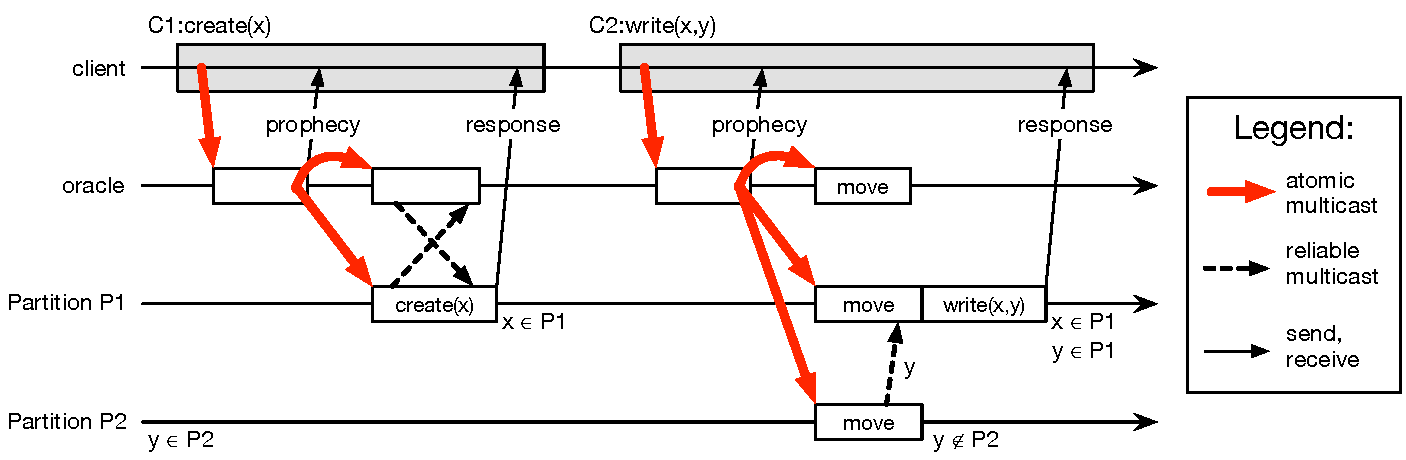
\includegraphics[width=\linewidth]{figures/dynastar}
\end{minipage}
\caption{Execution of a create (C1) and a write without client cache (C2) and with client cache (C3) in \dynastar.}
\label{fig:oracle_repartition}
\end{figure*}

Upon delivering a create (Task 2), the oracle updates its partition information.
The exchange of signals between the partition where the variable will be created
and the oracle ensures that interleaved executions between create and delete
commands will not lead to violations of linearizability (i.e., this is
essentially the execution of a multi-partition command involving the oracle and
a partition (Task 3) ~\cite{bezerra2014ssmr}). The oracle also keeps track of
the workload graph by receiving hints with variables (i.e., vertices in the
graph) and executing commands (i.e., edges in the graph). These hints can be
submitted by the clients or by the partitions, which collect data upon executing
commands and periodically inform the oracle (Task 4). The oracle computes a
partitioning plan of the graph and multicasts it to all servers and to itself.
Upon delivering a new partition plan, the oracle updates its location map
accordingly (Task 5).

To compute an optimized partitioning, the oracle uses a graph partitioner. A new
partitioning can be requested by the application, by a partition, or by the
oracle itself (e.g., upon delivering a certain number of hints). To determine
the destination partition of a set of variables, as part of a move, the oracle
uses its mapping of the current location of variables and the last computed
partitioning.

\subsubsection{The server process}

When a server delivers a command $C$, it first checks if it has all variables
needed by $C$. If the server has all such variables, it executes $C$ and sends
the response back to the client (Tasks 1a and 2 in
Algorithm~\ref{alg:dynastar-server_proxy}). If not all the variables needed by $C$ are in
that partition, the server runs a deterministic function to determine the
destination partition to execute $C$ (Task 1b). The function uses as input the
variables needed by $C$ and $C$ itself. In this case, each server that is in the
multicast group of $C$ but is not the destination partition sends all the needed
variables stored locally to the destination partition and waits to receive them
back. The destination partition waits for a message from other partitions. Once
all variables needed are available, the destination partition executes the $C$,
sends the response back to the client, and returns the variables to their
source. Periodically, the servers deliver a new partitioning plan from the
oracle (Task 3). Each server will send the variables to the designated
partition, as in the plan, and wait for variables from other partitions. Once a
server receives all variables, it updates its location map accordingly.
To determine the destination partition for a command, the servers uses the last
computed partitioning.

